\documentclass[a4paper, 16pt]{article}
\usepackage[UTF8]{ctex}
\usepackage{geometry}
\usepackage{graphicx}
\usepackage{setspace}
\usepackage{float}
\usepackage{listings}
\usepackage{xcolor}
\usepackage{multirow}
\lstset{
    numbers=left, 
    numberstyle= \tiny, 
    keywordstyle= \color{ blue!70},
    commentstyle= \color{red!50!green!50!blue!50}, 
    frame=shadowbox, % 阴影效果
    rulesepcolor= \color{ red!20!green!20!blue!20} ,
    escapeinside=``, % 英文分号中可写入中文
    xleftmargin=5em,xrightmargin=5em, aboveskip=2em,
    framexleftmargin=2em
} 
\geometry{left = 1.0 cm, right = 1.0cm, top = 2.0cm, bottom = 2.0cm	}
\title{编译原理第六章(三)}
\author{李鹏辉}

\begin{document}
\maketitle
1.(6.6.1)在图6-36的语法制导定义中添加处理下列控制流构造的规则

1) 一个repeat语句:$repeat\; S\; while\; B$


2)一个for循环语句:$for\; (S_1;\; B; S_2) S_3 $

\begin{table}[H]
\centering
\begin{tabular}{c|c}
\hline
\hline
PRODUCTION & SEMANTIC RULES \\
\multirow{4}{*}{$S \rightarrow repeat\; S\; while\; B$}
& $S = newlabel()$\\
& B.true = $S$ \\
& B.false = S.next \\
& $S.code = label(S) || S.code ||B.code || label(B.true)||gen('goto' S)||S.next$ \\
\hline
\multirow{8}{*}{$S \rightarrow for\; (S_1;\; B; S_2) S_3 $}
& $S_3 = newlabel()$\\
& $B = newlabel()$\\
& B.true = $S_3$ \\
& B.false = S.next \\
& $S_3.next = S_2$\\
& $S_2.next = B$\\
& $S.code = S_1.code || B.code || label(B.true)||S_3.code||S_2.code||gen('goto' B)||S.next$ \\
\hline
\hline
\end{tabular}
\end{table}

2.(6.7.1)使用图6-43的翻译方案翻译下列表达式。给出每个子表达式的truelist和falselist。你可以假设第一条被生成的指令地址是100

1) $a == b \;\&\&\; (c == d \;||\; e== f)$

\begin{figure}[H]
\centering
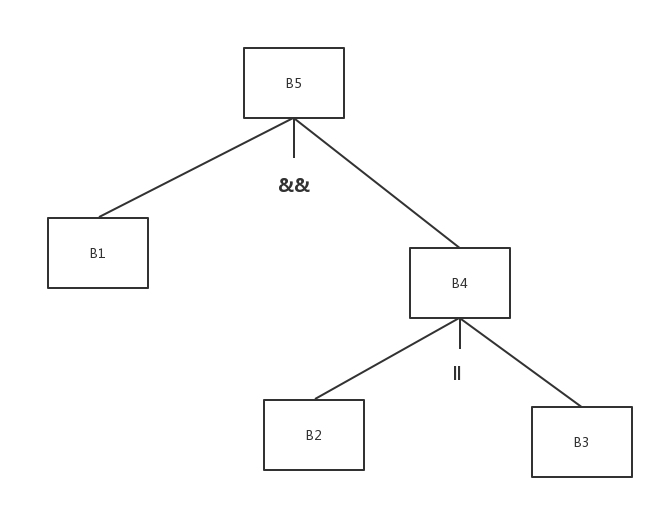
\includegraphics[scale=0.3]{chapter6_hw3_1}
\end{figure}

\begin{table}[H]
\centering
\begin{tabular}{c c}
100 & if(a == b) goto -\\
101 & goto -\\
102 &if (c ==d) goto -\\
103 &goto -\\
104 & if(e == f) goto -\\
105 & goto -\\
\end{tabular}
\end{table}

\begin{table}[H]
\centering
\begin{tabular}{c|c|c}
\hline
\hline
Block & T or F & \\
\hline
\multirow{2}{*}{$B_1$} 
&$B_1.truelist$ & 100\\
&$B_2.falselist$ &101\\
\hline
\multirow{2}{*}{$B_2$} 
&$B_2.truelist$&102\\
&$B_2.falselist$ &103\\
\hline
\multirow{2}{*}{$B3$} 
&$B_3.truelist$ &104\\
&$B_3.falselist$&105\\
\hline
\multirow{2}{*}{$B4$} 
&$B_4.truelist$&102,104\\
&$B_4.falselist$&105\\
\hline
\multirow{2}{*}{$B5$} 
&$B_5.truelist$&102,104\\
&$B_5.falselist$&101,105\\
\hline
\end{tabular}
\end{table}

\begin{table}[H]
\centering
\begin{tabular}{c c}
100 & if(a == b) goto 102\\
101 & goto false\\
102 &if (c ==d) goto true\\
103 &goto 104\\
104 & if(e == f) goto true\\
105 & goto false\\
\end{tabular}
\end{table}

2) $(a == b \;||\; c == d)\; ||\; e == f$

\begin{figure}[H]
\centering
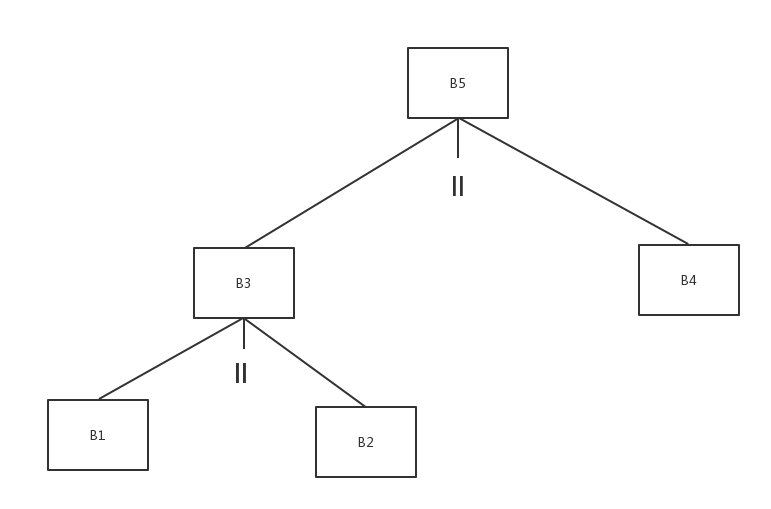
\includegraphics[scale=0.3]{chapter6_hw3_2}
\end{figure}

\begin{table}[H]
\centering
\begin{tabular}{c|c|c}
\hline
\hline
Block & T or F & \\
\hline
\multirow{2}{*}{$B_1$} 
&$B_1.truelist$ & 100\\
&$B_2.falselist$ &101\\
\hline
\multirow{2}{*}{$B_2$} 
&$B_2.truelist$&102\\
&$B_2.falselist$ &103\\
\hline
\multirow{2}{*}{$B3$} 
&$B_3.truelist$ &104\\
&$B_3.falselist$&105\\
\hline
\multirow{2}{*}{$B4$} 
&$B_4.truelist$&102,104\\
&$B_4.falselist$&103\\
\hline
\multirow{2}{*}{$B5$} 
&$B_5.truelist$&100, 102,104\\
&$B_5.falselist$&105\\
\hline
\end{tabular}
\end{table}

\begin{table}[H]
\centering
\begin{tabular}{c c}
100 & if(a == b) goto true\\
101 & goto 102\\
102 &if (c ==d) goto true\\
103 &goto 104\\
104 & if(e == f) goto true\\
105 & goto false\\
\end{tabular}
\end{table}

3) $(a == b \;\&\&\; c == d)\; \&\& \;e == f$


\begin{figure}[H]
\centering
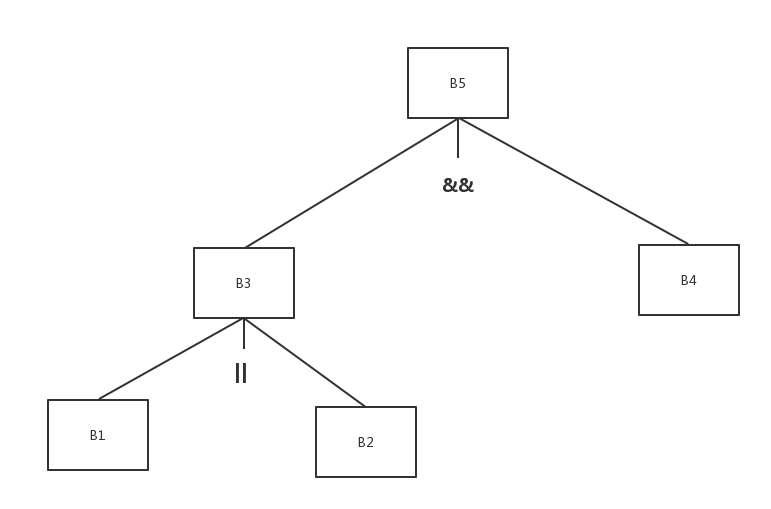
\includegraphics[scale=0.3]{chapter6_hw3_3}
\end{figure}

\begin{table}[H]
\centering
\begin{tabular}{c|c|c}
\hline
\hline
Block & T or F & \\
\hline
\multirow{2}{*}{$B_1$} 
&$B_1.truelist$ & 100\\
&$B_2.falselist$ &101\\
\hline
\multirow{2}{*}{$B_2$} 
&$B_2.truelist$&102\\
&$B_2.falselist$ &103\\
\hline
\multirow{2}{*}{$B3$} 
&$B_3.truelist$ &104\\
&$B_3.falselist$&105\\
\hline
\multirow{2}{*}{$B4$} 
&$B_4.truelist$&102\\
&$B_4.falselist$&101,103\\
\hline
\multirow{2}{*}{$B5$} 
&$B_5.truelist$&104\\
&$B_5.falselist$&101,103,105\\
\hline
\end{tabular}
\end{table}

\begin{table}[H]
\centering
\begin{tabular}{c c}
100 & if(a == b) goto 102\\
101 & goto false\\
102 &if (c ==d) goto 104\\
103 &goto false\\
104 & if(e == f) goto true\\
105 & goto false\\
\end{tabular}
\end{table}



\end{document}